\subsection{Vorstellung des Forschungsbeispiel SFB 637}
\label{sec:Forschungsbeispiel_SFB}
Im Rahmen dieser Ausarbeitung sollen die Möglichkeiten von selbststeuernden
Prozessen in der Produktionslogistik untersucht werden. Die Untersuchung wird
hierbei anhand eines Forschungsprojektes des Sonderforschungsbereichs 637
"`Selbststeuerung logistischer Prozesse – Ein Paradigmenwechsel und seine
Grenzen"' der Universität Bremen durchgeführt. Der Sonderforschungsbereich
befasst sich mit der Frage, auf welche Weise sich Modelle, Methoden und
Werkzeuge logistischer Prozesse abändern lassen, um eine dezentrale 
Selbststeuerung zu ermöglichen.

Bei dem zu untersuchenden Forschungsprojekt handelt es sich um eine
Demonstrationsplattform, die die vom Sonderforschungsbereich erarbeiteten
Selbststeuerungskonzepte anschaulich darstellen soll. Die
Demonstrationsplattform bildet ein Produktionsszenario für die Montage von
PKW-Rücklichtern ab. Der Montageprozess ermöglicht hierbei die Fertigung
verschiedener Produktvarianten der PKW-Rücklichter. Weiterhin können innerhalb
des Montageprozesses verschiedene Montagestationen flexibel durchlaufen werden.
In dem Produktionsprozess sind hierbei verschiedene Methoden der
Selbststeuerung umgesetzt. \abbildung{Montagestation} zeigt die einzelnen
Montagestationen der Demonstrationsplattform.

\begin{figure}[htb] 
\centering
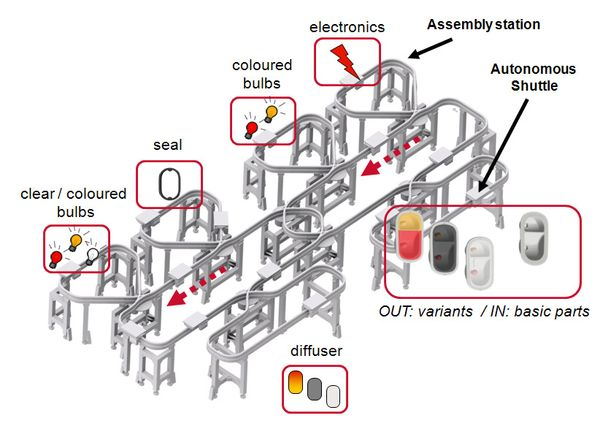
\includegraphics[width=1.0\textwidth]{Montage.jpg}
\caption[Montagestation]{Montagestationen der Demonstrationsplattform\protect\footnotemark}
\label{fig:Montagestation}
\end{figure}
\footnotetext{entnommen aus
\url{http://www.sfb637.uni-bremen.de/produktions_logistik.html [Stand
 17.03.2014]}}
%TODO: Wo kommt das Bild her?

Die Demonstrationsplattform besteht aus einem Einschienensystem, auf dem sich
mehrere Transportplattformen, sogenannte Shuttles, autonom bewegen können. Die
Shuttles transportieren die Rücklichter einzeln durch das Montagesystem. Zu
Beginn des Montageprozesses wird ein Reflektor-Gussteil, welches das
Ausgangsbauteil der Montage darstellt, auf dem Shuttle angebracht. In jedes
dieser Reflektor-Gussteile wurde dabei ein RFID-Transponder\footnote{engl.
radio-frequency identification} integriert, welcher die eindeutige
Identifikation des Bauteils über den gesamten Montageprozess hinweg ermöglicht.

Im Verlauf des Montageprozesses wird das Ausgangsbauteil an verschiedenen
Montagestationen um die Komponenten Kabelbaum, Leuchtmittel, Dichtung und
Blende erweitert. Die Reihenfolge, in der die einzelnen Komponenten an den
Reflektor angebracht werden können, ist dabei flexibel. Es müssen jedoch
bestimmte Abhängigkeiten eingehalten werden. So müssen beispielsweise 
Leuchtmittel und Dichtung vor der Blende montiert werden. Der Kabelbaum kann
hingegen zu jeder Zeit an dem Reflektor angebracht werden. Die hierdurch
entstehenden Abhängigkeiten sind in einem sogenannten Variantenkorridor
abgebildet. (siehe \abbildung{Variantenkorridor})

\begin{figure}[htb] 
\centering
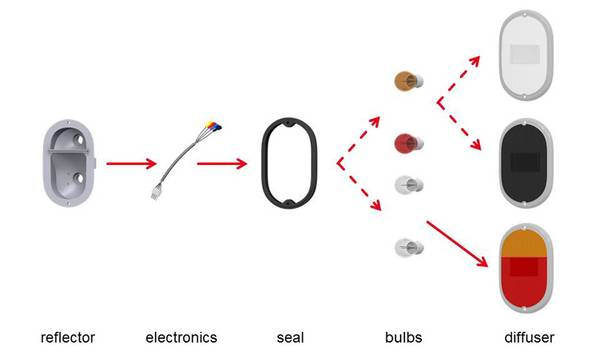
\includegraphics[width=1.0\textwidth]{Variantenkorridor.jpg}
\caption[Variantenkorridor]{Variantenkorridor\protect\footnotemark}
\label{fig:Variantenkorridor}
\end{figure}
\footnotetext{entnommen aus
\url{http://www.sfb637.uni-bremen.de/produktions_logistik.html [Stand
 17.03.2014]}}
%TODO: Wo kommt das Bild her?

Durch die Möglichkeit, die einzelnen Rücklichter eindeutig zu identifizieren,
können diese konkret einer Produktvariante und einem Auftrag zugeordnet und
somit direkt in die Produktionsplanung einbezogen werden. Jedes Produkt wird
innerhalb des Montagesystems durch einen sogenannten Softwareagenten
repräsentiert. Dieser kann innerhalb des Montageprozesses auf kurzfristige
Änderungen der Auftragslage reagieren. In dem Montagesystem kann das einzelne 
Produkt so bei einer Stornierung eines Auftrags direkt einem anderen
Kundenauftrag zugeordnet werden. Hierbei kann für das konkrete Produkt
gegebenenfalls sogar eine andere als die zuvor angedachte Produktausführung
durch den Softwareagenten festgelegt werden.


